\documentclass[11pt,a4paper]{article}

\usepackage[margin=2.5cm]{geometry}
\usepackage[utf8]{inputenc}
\usepackage[T1]{fontenc}
\usepackage{lmodern}
\usepackage{amsmath,amssymb}
\usepackage{graphicx}
\graphicspath{{figures/}{constraint_propagation_backtracking/}{simulated_annealing/}{genetic_algorithm/}}
\usepackage{booktabs}
\usepackage{array}
\usepackage{enumitem}
\usepackage{float}
\usepackage[section]{placeins}
\usepackage{algorithm}
\usepackage{algpseudocode}
\usepackage{tcolorbox}
\usepackage[hidelinks]{hyperref}

\setlength{\parskip}{4pt}
\renewcommand{\algorithmicrequire}{\textbf{Input:}}
\renewcommand{\algorithmicensure}{\textbf{Output:}}

\begin{document}

\begin{titlepage}
  \centering
  
\includegraphics[width=0.35\textwidth]{logo.png}\par
  \vspace{1.5cm}
  {\large Università Ca' Foscari Venezia\par}
  {\large Dipartimento di Scienze Ambientali, Informatica e Statistica\par}
  \vspace{1.5cm}
  {\Large Foundations of Artificial Intelligence\par}
  \vspace{1cm}
  \rule{\textwidth}{0.4pt}\par
  \vspace{0.4cm}
  {\huge\bfseries The $N\times N$ Magic Square Problem\par}
  \vspace{0.3cm}
  {\large Constraint Propagation and Backtracking,\\
          Simulated Annealing, Genetic Algorithms\par}
  \vspace{0.4cm}
  \rule{\textwidth}{0.4pt}\par
  \vfill
  {\large
  \begin{tabular}{rl}
    Student: & Wafaa Bajjouk \\
    Student ID: & 916145 \\
    Professor: & Andrea Torsello \\
    Academic year: & 2026/2027 \\
  \end{tabular}\par}
  \vspace{1cm}
  {\large \today\par}
\end{titlepage}

\tableofcontents
\newpage

\section{Introduction}

The goal is to fill an $N\times N$ grid with the numbers $1,\dots,N^2$
so that every row, every column and both diagonals have the same sum $M$,
possibly with some cells already given. There are $(N^2)!$ ways to fill
the grid, so I need search methods that do not try them all. I use
three methods from the course:
\begin{itemize}[nosep]
  \item \textbf{Backtracking with constraint propagation:} fill one cell
        at a time, remove the values that can no longer fit, and go back
        when a cell has no value left.
  \item \textbf{Simulated annealing:} start from a full grid and swap two
        cells at a time, sometimes accepting a worse grid to escape local
        minima.
  \item \textbf{Genetic algorithm:} keep a population of full grids and
        build new ones by selection, crossover and mutation. I also tried
        the PyGAD library for it, but it was slower, so I kept my own code
        (Section~\ref{sec:m3}).
\end{itemize}
For each method I follow the same process: I describe the theory and
the pseudocode, test it on one $4\times4$ puzzle, and then run it on
squares of growing size, with and without given cells, with a limit of
10\,s per run. Finally I compare the three methods on the same puzzles.
The code of the methods and of all the experiments, with the raw results,
is in the repository
\url{https://github.com/WafaaBajjouk/Foundation_AI_assignments}.
Sections~\ref{sec:m1}--\ref{sec:m3} present the methods,
Section~\ref{sec:compare} compares them and Section~\ref{sec:conclusions}
concludes.

\section{Problem statement}
\label{sec:problem}

A magic square of order $N$ is an $N\times N$ grid containing each of the
numbers $1,\dots,N^2$ once, where every row, column and main diagonal
has the same sum $M$. The numbers add up to $N^2(N^2+1)/2$ and the $N$
rows share this total equally, so
\[
M=\frac{N(N^2+1)}{2}\qquad(M=15 \text{ for } N=3,\ M=34 \text{ for } N=4).
\]

Let $x_{ij}$ be the value of cell $(i,j)$, $\mathcal{L}$ the set of the
$2N+2$ lines (rows, columns, two diagonals), and $G$ the set of given
cells with values $g_{ij}$. I look for $x_{ij}$ such that
\begin{align*}
& x_{ij}\in\{1,\dots,N^2\}, && x_{ij}\neq x_{kl}\ \ \forall (i,j)\neq(k,l),\\
& \textstyle\sum_{(i,j)\in L}x_{ij}=M\ \ \forall L\in\mathcal{L}, && x_{ij}=g_{ij}\ \ \forall (i,j)\in G.
\end{align*}
There are $(N^2)!$ ways to fill the grid. Trying them all is still
feasible for $N=3$ ($9!=362\,880$), but it quickly becomes impractical as
$N$ grows: already $25!\approx1.6\cdot10^{25}$ for $N=5$.

\textbf{Code and data.} All the code and the raw results are in the
repository below, with one folder per method containing its notebook,
its results (CSV) and its plots:
\begin{center}
\url{https://github.com/WafaaBajjouk/Foundation_AI_assignments}
\end{center}
\newpage
\section{Method 1: Constraint propagation and backtracking}
\label{sec:m1}

\subsection{The problem as a constraint satisfaction problem}

The goal state itself is the solution, so the problem is a constraint
satisfaction problem \cite{slides,aima}:
\begin{itemize}[nosep]
  \item \textbf{variables:} the $N^2$ cells $x_{ij}$;
  \item \textbf{domains:} $\{g_{ij}\}$ for a given cell, $\{1,\dots,N^2\}$ otherwise;
  \item \textbf{constraints:} all values different, every line sums to $M$.
\end{itemize}
It is solved by two ideas together: crossing off impossible numbers (propagation) and trying values (search).

\subsection{Constraint propagation}

Propagation deletes values that cannot belong to any solution. An arc
$(v_i,v_j)$ is arc consistent if
\[
\forall x\in D_i\ \ \exists y\in D_j \text{ such that } (x,y) \text{ satisfies the constraint};
\]
values of $D_i$ without such a $y$ are deleted.

\textbf{All different.} If $D_a=\{v\}$, then $v$ is deleted from every
other domain.

\textbf{Line sums.} Let a line have $k$ free cells that must sum to $R$,
and let $U$ be the values still possible in them. A value $v$ is deleted if
\[
R-v<lo(v)\quad\text{or}\quad R-v>hi(v),
\]
where $lo(v)$ and $hi(v)$ are the sums of the $k-1$ smallest and largest
values of $U\setminus\{v\}$. If $k=1$, the last cell must be $R$.

\textbf{Forward checking vs.\ full propagation.} The two choices differ
in how much they propagate after a value is assigned:
\begin{itemize}[nosep]
  \item \textbf{Forward checking (FC):} only the constraints that involve
        the cell just assigned are revised, once. It is fast but removes
        few values.
  \item \textbf{Full propagation (AC):} the deletions above are repeated
        on all constraints until no domain changes (a fixed point). For the
        pairwise constraints $x_a\neq x_b$ this gives arc consistency, but
        it is weaker than full propagation of the global all-different
        constraint; for the line sums only the bound test is applied. It is slower at each step but
        removes more values.
\end{itemize}

\begin{algorithm}[H]
\small
\caption{Constraint propagation}
\label{alg:prop}
\begin{algorithmic}[1]
\Function{ForwardCheck}{$D,c,v$}
  \State delete $v$ from every $D_x$, $x\neq c$
  \If{some $D_x=\emptyset$} \State \Return failure \EndIf
  \For{each line $L$ containing $c$}
    \If{\Call{ReviseLine}{$D,L$} $=$ failure} \State \Return failure \EndIf
  \EndFor
  \State \Return ok
\EndFunction
\Statex
\Function{Propagate}{$D$} \Comment{full propagation (AC)}
  \Repeat
    \State $s\gets\sum_x|D_x|$
    \If{two cells are fixed to the same value} \State \Return failure \EndIf
    \State delete the values of the fixed cells from all other domains
    \If{some $D_x=\emptyset$} \State \Return failure \EndIf
    \For{each line $L\in\mathcal{L}$}
      \If{\Call{ReviseLine}{$D,L$} $=$ failure} \State \Return failure \EndIf
    \EndFor
  \Until{$\sum_x|D_x|=s$}
  \State \Return ok
\EndFunction
\Statex
\Function{ReviseLine}{$D,L$}
  \State $F\gets$ free cells of $L$; \ $k\gets|F|$; \ $R\gets M-$ sum of the fixed cells of $L$
  \If{$k=0$} \State \Return ok if $R=0$, else failure \EndIf
  \If{$k=1$}
    \State $D_x\gets D_x\cap\{R\}$ for the free cell $x$
  \Else
    \State $U\gets\bigcup_{x\in F}D_x$
    \If{$|U|<k$} \State \Return failure \EndIf
    \For{each $x\in F$ and each $v\in D_x$}
      \If{$R-v<lo(v)$ or $R-v>hi(v)$} \State $D_x\gets D_x\setminus\{v\}$ \EndIf
    \EndFor
  \EndIf
  \State \Return failure if some $D_x=\emptyset$, $x\in F$, else ok
\EndFunction
\end{algorithmic}
\end{algorithm}

\subsection{Backtracking}

Backtracking is a depth-first search on partial assignments: a variable
gets a tentative value, the effect is propagated, and if a domain becomes
empty the value is undone. The order is chosen during the search:
\begin{itemize}[nosep]
  \item \textbf{most constrained variable:} the variable with the fewest
        legal values;
  \item \textbf{least constraining value (LCV):} the value that removes
        the fewest values from the other domains (the baseline is
        ascending order).
\end{itemize}

\begin{algorithm}[H]
\small
\caption{Backtracking with constraint propagation}
\label{alg:bt}
\begin{algorithmic}[1]
\Function{BacktrackingSearch}{$G, g$}
  \State $D_c\gets\{g_c\}$ if $c\in G$, else $D_c\gets\{1,\dots,N^2\}$
  \If{\Call{Propagate}{$D$} $=$ failure} \State \Return failure \EndIf
  \State \Return \Call{Backtrack}{$D$}
\EndFunction
\Statex
\Function{Backtrack}{$D$}
  \If{$|D_c|=1$ for every cell $c$}
    \State \Return $D$ if all values differ and all lines sum to $M$, else failure
  \EndIf
  \State $c\gets$ cell with $|D_c|>1$ and smallest $|D_c|$
  \For{each $v\in D_c$, in LCV or ascending order}
    \State $D'\gets$ copy of $D$; \ $D'_c\gets\{v\}$
    \If{\Call{ForwardCheck}{$D',c,v$} (FC) or \Call{Propagate}{$D'$} (AC) $\neq$ failure}
      \State $result\gets$ \Call{Backtrack}{$D'$}
      \If{$result\neq$ failure} \State \Return $result$ \EndIf
    \EndIf
  \EndFor
  \State \Return failure
\EndFunction
\end{algorithmic}
\end{algorithm}

\subsection{Properties}

\begin{itemize}[nosep]
  \item \textbf{Completeness:} backtracking explores a finite tree of
        depth $d=N^2$. Without a time limit it always finds a solution if
        one exists, and reports failure if the givens make the problem
        impossible.
  \item \textbf{Time:} the search tree has $O(b^d)$ nodes, where $b$ is
        the branching factor (the number of values tried per cell). The
        real time also includes the propagation and value-ordering work
        done at each node. It grows exponentially with the number of cells.
  \item \textbf{Memory:} depth-first search keeps only the current path,
        but at each of the $d=N^2$ levels my search stores a copy of the
        $N^2$ domains, each with at most $N^2$ values, so the memory is
        $O(N^6)$ in the worst case.
  \item \textbf{Effect of propagation:} it never removes a solution; it
        only reduces $b$, so fewer nodes are explored.
\end{itemize}

\noindent From these properties I expect that:
\begin{itemize}[nosep]
  \item AC explores fewer nodes than FC;
  \item the time grows exponentially with $N$;
  \item given cells shrink the domains from the start, which should help,
        although they also leave fewer valid solutions.
\end{itemize}

\subsection{Experimental setup}

Instances are built from a known magic square of order $N$ (Siamese
method for odd $N$, standard constructions for even $N$), randomly
rotated or mirrored; a random subset of its cells is kept as givens, so the givens are
always consistent. The number of given cells is $\lfloor 0.2N^2\rfloor$;
puzzles are sampled from rotations and reflections of one constructed
magic square per size, which limits instance diversity.

\textbf{Experiment 1a.} One $4\times4$ instance with three given cells
($x_{11}=13$, $x_{13}=12$, $x_{24}=15$), solved with the four
combinations of FC/AC and ascending/LCV. I record nodes, backtracks and
time, and check that every returned square is magic and keeps the givens.

\textbf{Experiment 1b.} The same four combinations for $N=3,\dots,7$,
with no givens or $20\%$ of the cells given, 5 instances each (200 runs),
time limit 10\,s per run. I record the percentage solved and the median
time. Runs have a nominal 10\,s limit. A run that reaches it counts as not
solved; its actual elapsed time is kept, including the small overshoot of
the deadline (10.000--10.006\,s), so failed runs are included in the
median times and must be
read together with the percentage solved. Without givens every instance is the empty grid and the search is
deterministic, so the 5 runs explore the same tree and differ only in
running time. All runs use an M1 with 16\,GB of RAM and Python~3.

\textbf{Code and data.} Folder \nolinkurl{constraint_propagation_backtracking/}
of the repository:
\begin{itemize}[nosep]
  \item notebook: \nolinkurl{constraint_propagation_backtracking.ipynb};
  \item raw results of Experiment 1b: \nolinkurl{results_alg1.csv}.
\end{itemize}

\subsection{Results}

\begin{table}[H]
\centering
\begin{tabular}{@{}llrrr@{}}
\toprule
Propagation & Value order & Nodes & Backtracks & Time (s) \\
\midrule
FC & ascending & 2286 & 2280 & 0.040 \\
FC & LCV & 761 & 755 & 0.020 \\
AC & ascending & 100 & 97 & 0.013 \\
AC & LCV & 37 & 34 & 0.012 \\
\bottomrule
\end{tabular}
\caption{Experiment 1a. Every run returns a valid magic square that
keeps the givens; the four settings do not all return the same square.}
\label{tab:alg1demo}
\end{table}

\begin{figure}[H]
\centering
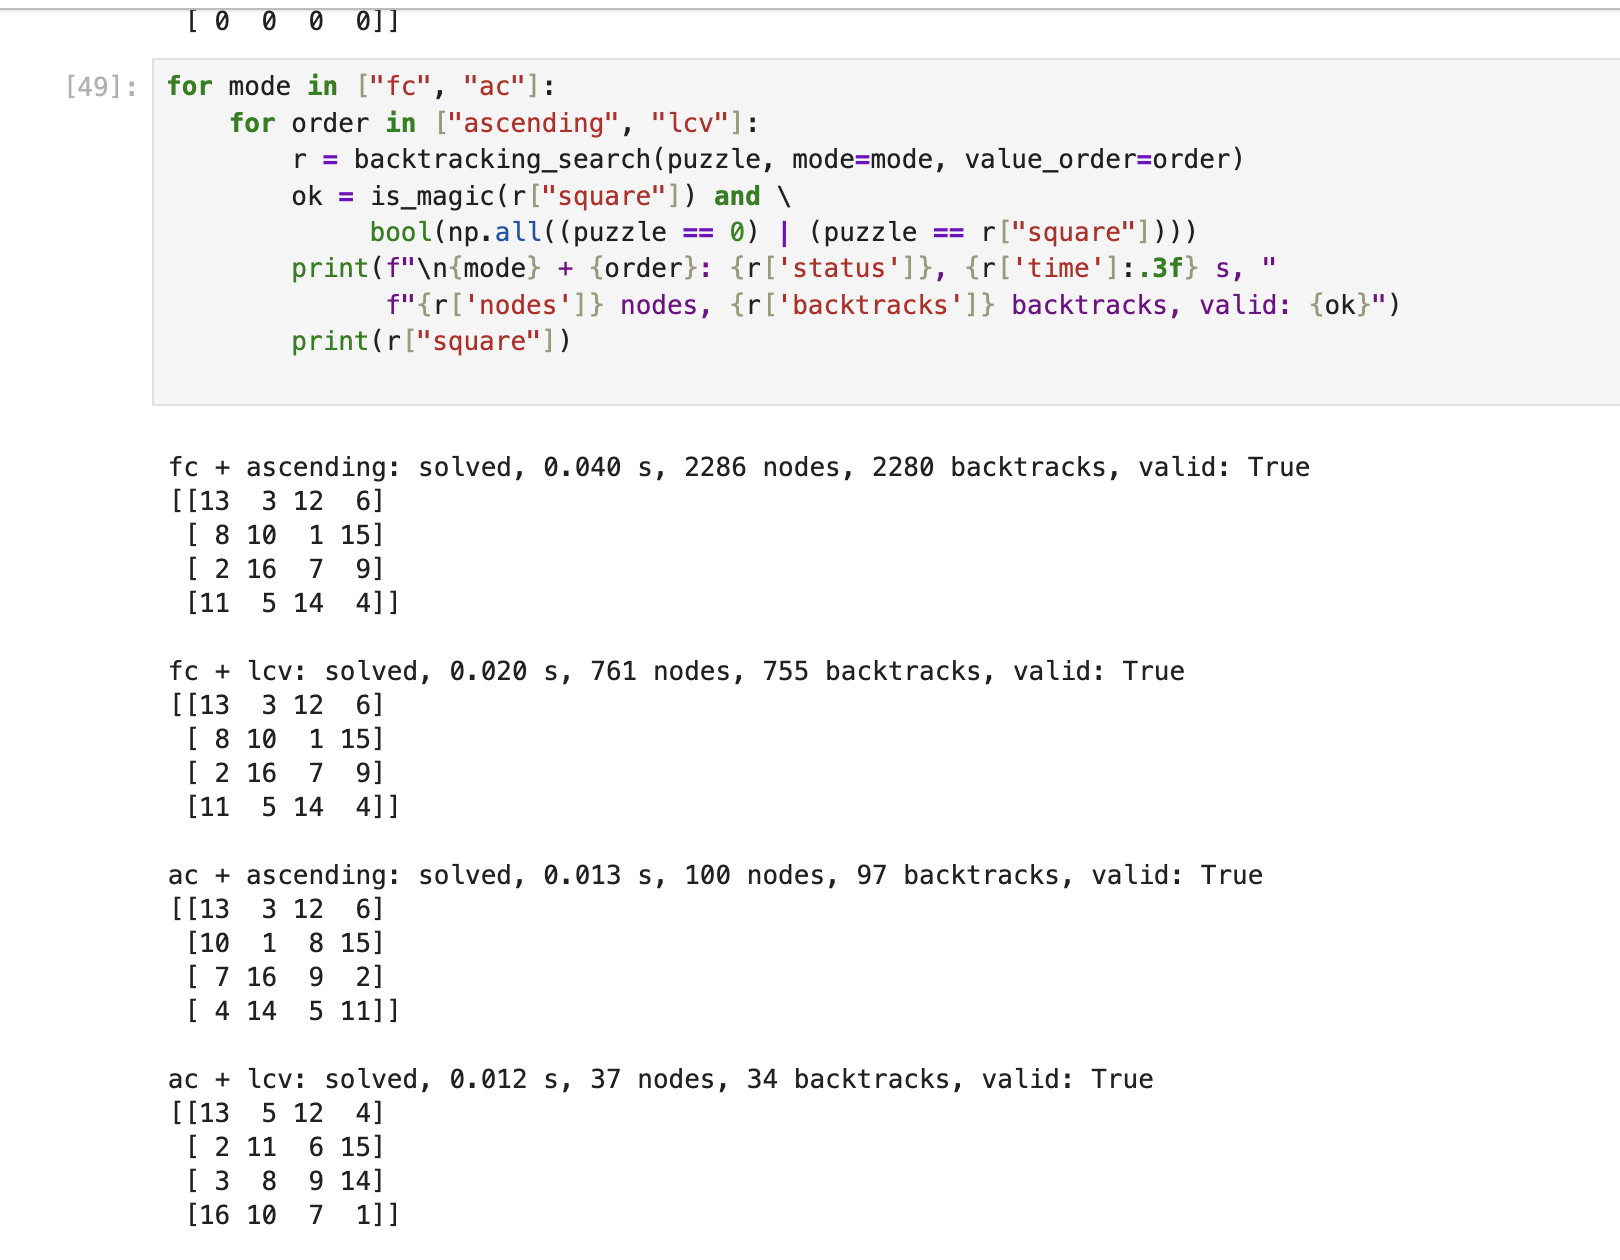
\includegraphics[width=0.5\textwidth]{alg1_demo.png}
\caption{Notebook output of Experiment 1a.}
\label{fig:alg1demo}
\end{figure}

\begin{table}[H]
\centering
\small
\begin{tabular}{@{}l rrrrr c rrrrr@{}}
\toprule
 & \multicolumn{5}{c}{solved (\%), no givens} && \multicolumn{5}{c}{solved (\%), 20\% given} \\
\cmidrule{2-6}\cmidrule{8-12}
$N$ & 3 & 4 & 5 & 6 & 7 && 3 & 4 & 5 & 6 & 7 \\
\midrule
FC + ascending & 100 & 100 & 0   & 0   & 0 && 100 & 100 & 40  & 0   & 0  \\
FC + LCV       & 100 & 100 & 0   & 0   & 0 && 100 & 100 & 100 & 20  & 0  \\
AC + ascending & 100 & 100 & 100 & 0   & 0 && 100 & 100 & 100 & 80  & 0  \\
AC + LCV       & 100 & 100 & 100 & 100 & 0 && 100 & 100 & 100 & 100 & 60 \\
\midrule
 & \multicolumn{5}{c}{median time (s), no givens} && \multicolumn{5}{c}{median time (s), 20\% given} \\
\cmidrule{2-6}\cmidrule{8-12}
FC + ascending & 0.001 & 0.004 & $\geq$10 & $\geq$10 & $\geq$10 && 0.000 & 0.002 & $\geq$10 & $\geq$10 & $\geq$10 \\
FC + LCV       & 0.002 & 0.025 & $\geq$10 & $\geq$10 & $\geq$10 && 0.000 & 0.002 & 3.56  & $\geq$10 & $\geq$10 \\
AC + ascending & 0.000 & 0.003 & 0.32 & $\geq$10 & $\geq$10 && 0.000 & 0.001 & 0.37  & 0.20  & $\geq$10 \\
AC + LCV       & 0.007 & 0.062 & 0.22 & 0.47  & $\geq$10 && 0.001 & 0.005 & 1.23  & 3.12  & 7.66  \\
\bottomrule
\end{tabular}
\caption{Experiment 1b ($\geq$10: the median run reached the 10\,s limit;
failed runs take about 10\,s). Raw data:
\nolinkurl{results_alg1.csv}.}
\label{tab:alg1n}
\end{table}

\begin{figure}[H]
\centering
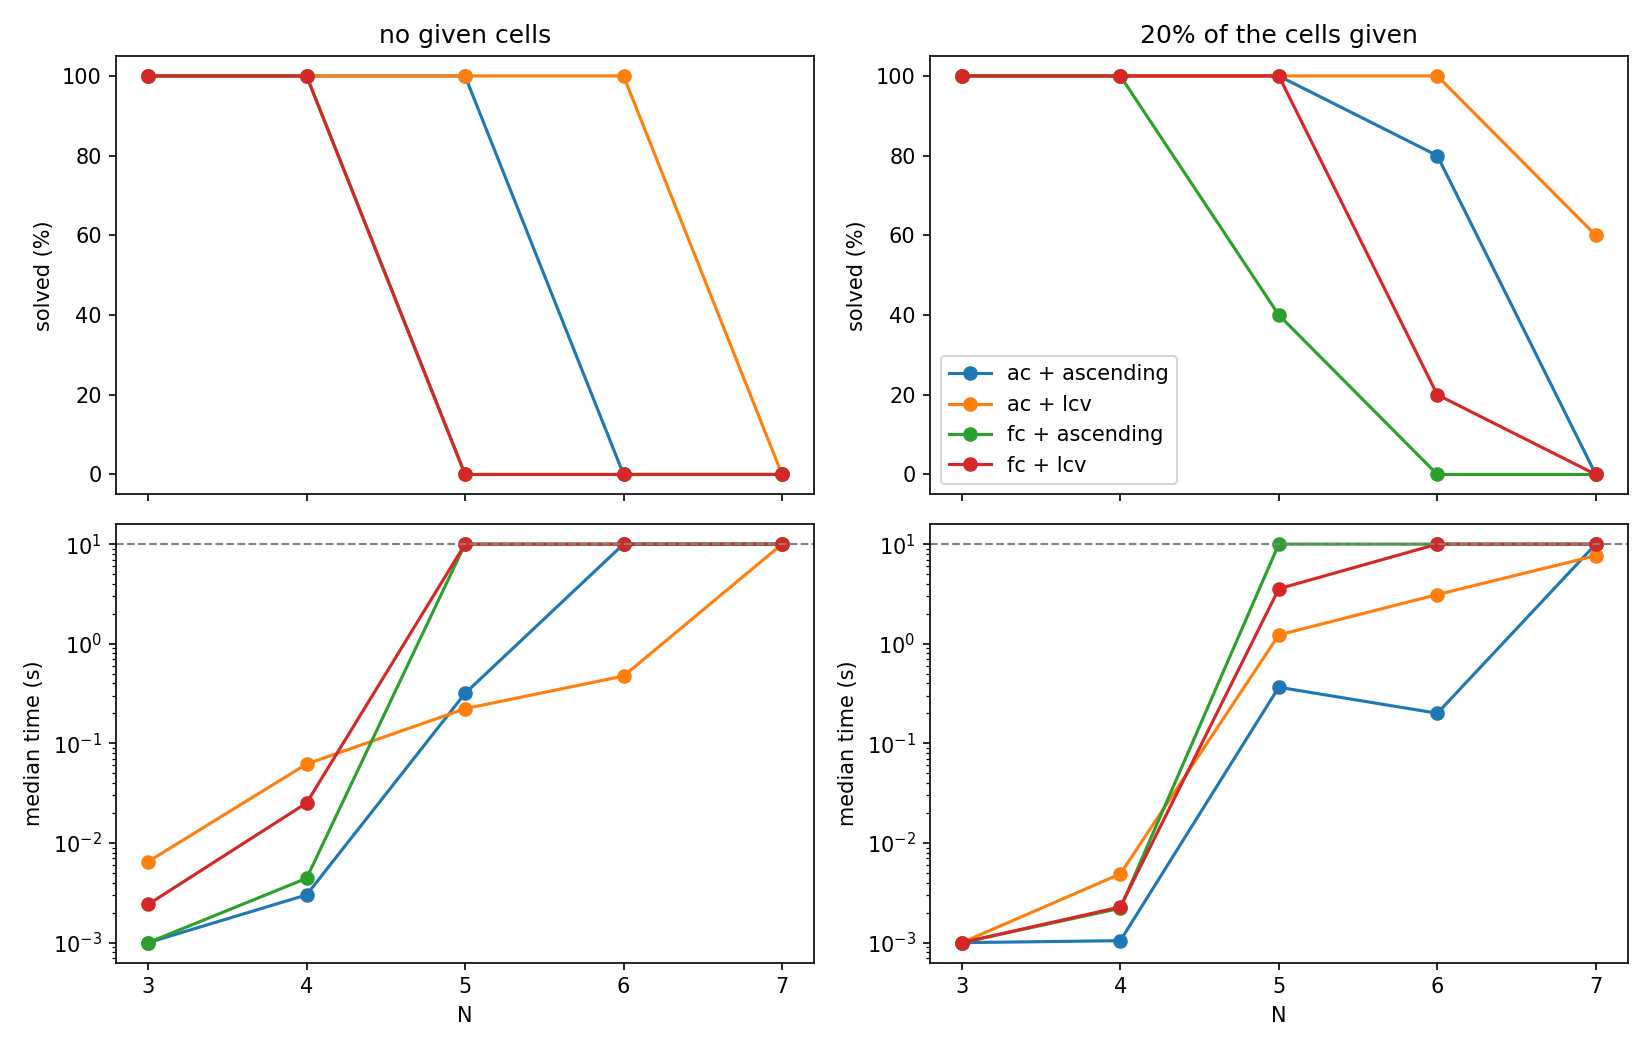
\includegraphics[width=\textwidth]{alg1_time.png}
\caption{Experiment 1b: solved instances and median time (log scale);
dashed line: 10\,s limit. In the top-left panel two curves overlap
(FC + ascending, FC + LCV).}
\label{fig:alg1n}
\end{figure}

\textbf{Analysis.}
\begin{itemize}[nosep]
  \item At $N=5$ without givens, AC with LCV solves the puzzle with $394$
        nodes, while FC with ascending order explores about $1.2$ million
        nodes in 10\,s without finding a solution. This gain comes from
        both changes together, stronger propagation and a better value
        order, not from propagation alone.
  \item AC with LCV is the best combination: the only one that solves all
        instances up to $N=6$ and some at $N=7$. LCV has a cost, since it
        runs one propagation for every candidate value: at $N=4$ without
        givens AC with LCV takes 0.062\,s against 0.003\,s with ascending
        order, and it pays off only from $N=5$.
  \item The time grows very fast with $N$; at $N=7$ almost every run
        reaches the limit.
  \item Givens help at $N=7$ (60\% solved against 0\%) but slow AC with
        LCV down at $N=5,6$ (1.23\,s against 0.22\,s, 3.12\,s against
        0.47\,s); a possible reason is that fewer squares are
        valid solutions.
\end{itemize}
Runs that end close to the limit can change between executions, since
they depend on the speed of the machine: FC with ascending order solved
$N=5$ without givens in about 9\,s in an earlier run, but reached the
limit in this one.
Method 1 is exact; on the tested instances and with a 10\,s limit, AC
with LCV solves every instance only up to $N=6$.
AC with LCV is used in the comparison of Section~\ref{sec:compare}.

\section{Method 2: Simulated Annealing}
\label{sec:m2}

\subsection{The problem as an optimization problem}

Local search turns the CSP into an optimization problem
\cite{slides}: I define an objective function that is positive, and $0$
if and only if all constraints are satisfied, and minimise it by moving
between neighbouring states.
\begin{itemize}[nosep]
  \item \textbf{state:} a complete grid with each of $1,\dots,N^2$ once and
        the given cells in place, so all values are always different;
  \item \textbf{objective (energy):}
        \[
        f(s)=\sum_{L\in\mathcal{L}}\Big|\sum_{(i,j)\in L}x_{ij}-M\Big|,
        \]
        which is $0$ if and only if $s$ is a magic square;
  \item \textbf{neighbour:} swap the values of two free cells.
\end{itemize}

\subsection{Simulated annealing}

Hill climbing always moves to a better state, so it stops in local
minima. Simulated annealing picks a random neighbour $s^*$ and, with
$\Delta=f(s^*)-f(s)$:
\begin{itemize}[nosep]
  \item \textbf{if $\Delta<0$:} always moves to $s^*$;
  \item \textbf{otherwise:} moves to $s^*$ with probability $e^{-\Delta/T}$.
\end{itemize}
The temperature $T$ starts high, so worse moves are often accepted, and
decreases, so that at the end almost only better moves are accepted.
\begin{itemize}[nosep]
  \item \textbf{schedule:} $T_0$ is the mean increase of $f$ over the
        worsening swaps among 200 random ones; then $T\gets\alpha T$ at each step, down to $0.01$ after
        $L=2000N^2$ steps;
  \item \textbf{restart:} if a run ends with $f(s)>0$, the search restarts
        from a new random state, until the time limit.
\end{itemize}

\begin{algorithm}[H]
\small
\caption{Simulated annealing}
\label{alg:sa}
\begin{algorithmic}[1]
\Function{SimulatedAnnealing}{$G, g$}
  \Repeat
    \State $s\gets$ givens in place, the other values shuffled into the free cells
    \State $T\gets T_0$; \ $\alpha\gets(0.01/T_0)^{1/L}$
    \For{$k=1,\dots,L$}
      \If{$f(s)=0$} \State \Return $s$ \EndIf
      \State $s^*\gets s$ with two random free cells swapped
      \State $\Delta\gets f(s^*)-f(s)$
      \If{$\Delta<0$ \textbf{or} $random()<e^{-\Delta/T}$} \State $s\gets s^*$ \EndIf
      \State $T\gets\alpha T$
    \EndFor
  \Until{time limit reached}
  \State \Return failure
\EndFunction
\end{algorithmic}
\end{algorithm}

\subsection{Properties}

\begin{itemize}[nosep]
  \item \textbf{Not complete:} the search is random, so it can miss a
        solution and cannot prove that a set of givens has none.
  \item \textbf{Convergence:} if $T$ decreases slowly enough, the global
        optimum is reached with probability approaching $1$
        \cite{slides,kirkpatrick}.
  \item \textbf{Cost per step:} I keep the sum of every line in memory
        and update it after each accepted swap. A swap changes at most 8
        lines (the row, column and diagonals of the two cells), so with
        these stored sums $\Delta$ is computed in constant time; computing
        the same lines again from their cells would cost $O(N)$. The memory
        is $O(N^2)$.
\end{itemize}

\noindent From these properties I expect that:
\begin{itemize}[nosep]
  \item SA reaches larger $N$ than backtracking;
  \item some runs end in a local minimum, so restarts will be used;
  \item given cells may make the problem harder: fewer squares are valid
        solutions, and SA can only move the free values, without pruning
        them as backtracking does.
\end{itemize}

\subsection{Experimental setup}

The instances are built as for Method 1.

\textbf{Experiment 2a.} The $4\times4$ instance of Experiment 1a, solved
once; I record the energy during the search.

\textbf{Experiment 2b.} $N=3,\dots,10$, with no givens or $20\%$ of the
cells given. For each case I use 3 puzzles and 3 independent runs per
puzzle, with separate seeds for the puzzle and the run (9 runs per point,
144 in total), so that the difficulty of the puzzle and the randomness of
SA are not mixed. The time limit is 10\,s per run and is checked every
1000 steps. I record the percentage solved, the median time (failed
runs take about 10\,s, as for Method 1) and the median number of restarts.
Same machine as Method 1.

\textbf{Why up to $N=10$.} Method 1 was stopped at $N=7$, where almost
every run already reached the time limit. SA still solves every instance
without givens at $N=8$ in preliminary runs, so the sizes are extended
to $N=10$ to find where its limit is.

\textbf{Code and data.} Folder \nolinkurl{simulated_annealing/} of the
repository:
\begin{itemize}[nosep]
  \item notebook: \nolinkurl{simulated_annealing.ipynb};
  \item raw results of Experiment 2b: \nolinkurl{results_sa.csv}.
\end{itemize}

\subsection{Results}

\textbf{Experiment 2a.} The $4\times4$ instance is solved in
$0.036$\,s and $6181$ iterations, without restarts. The square found
keeps the givens and is the same one found by Method 1 with AC and
ascending order.

\begin{figure}[H]
\centering
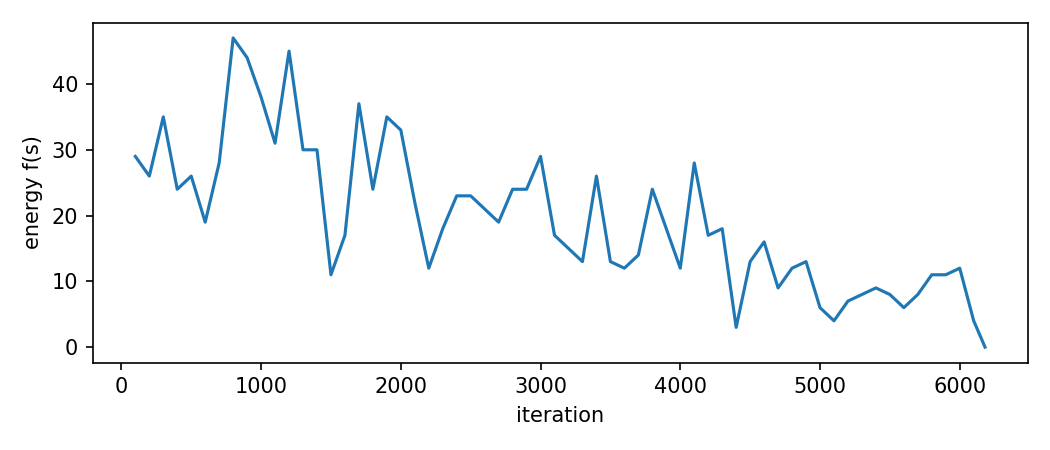
\includegraphics[width=0.75\textwidth]{sa_energy.png}
\caption{Experiment 2a: energy during the search. At high temperature
worse states are often accepted; as $T$ decreases the energy falls to $0$.}
\label{fig:saenergy}
\end{figure}

\textbf{Experiment 2b.}

\begin{table}[H]
\centering
\small
\begin{tabular}{@{}l rrrrrrrr@{}}
\toprule
$N$ & 3 & 4 & 5 & 6 & 7 & 8 & 9 & 10 \\
\midrule
solved (\%), no givens   & 100 & 100 & 100 & 100 & 100 & 100 & 78 & 100 \\
solved (\%), 20\% given  & 100 & 100 & 89  & 67  & 67  & 44  & 33 & 56  \\
\midrule
median time (s), no givens  & 0.004 & 0.04 & 1.42 & 1.51 & 1.33 & 1.44 & 2.22  & 1.99 \\
median time (s), 20\% given & 0.002 & 0.03 & 3.13 & 8.85 & 6.05 & $\geq$10 & $\geq$10 & 7.25 \\
\midrule
median restarts, no givens  & 0 & 0 & 7  & 5  & 3  & 2  & 3  & 2 \\
median restarts, 20\% given & 0 & 0 & 16 & 33 & 16 & 21 & 16 & 9 \\
\bottomrule
\end{tabular}
\caption{Experiment 2b (9 runs per point; $\geq$10: the median run reached
the 10\,s limit; failed runs take about 10\,s). Raw
data: \nolinkurl{results_sa.csv}.}
\label{tab:sa}
\end{table}

\begin{figure}[H]
\centering
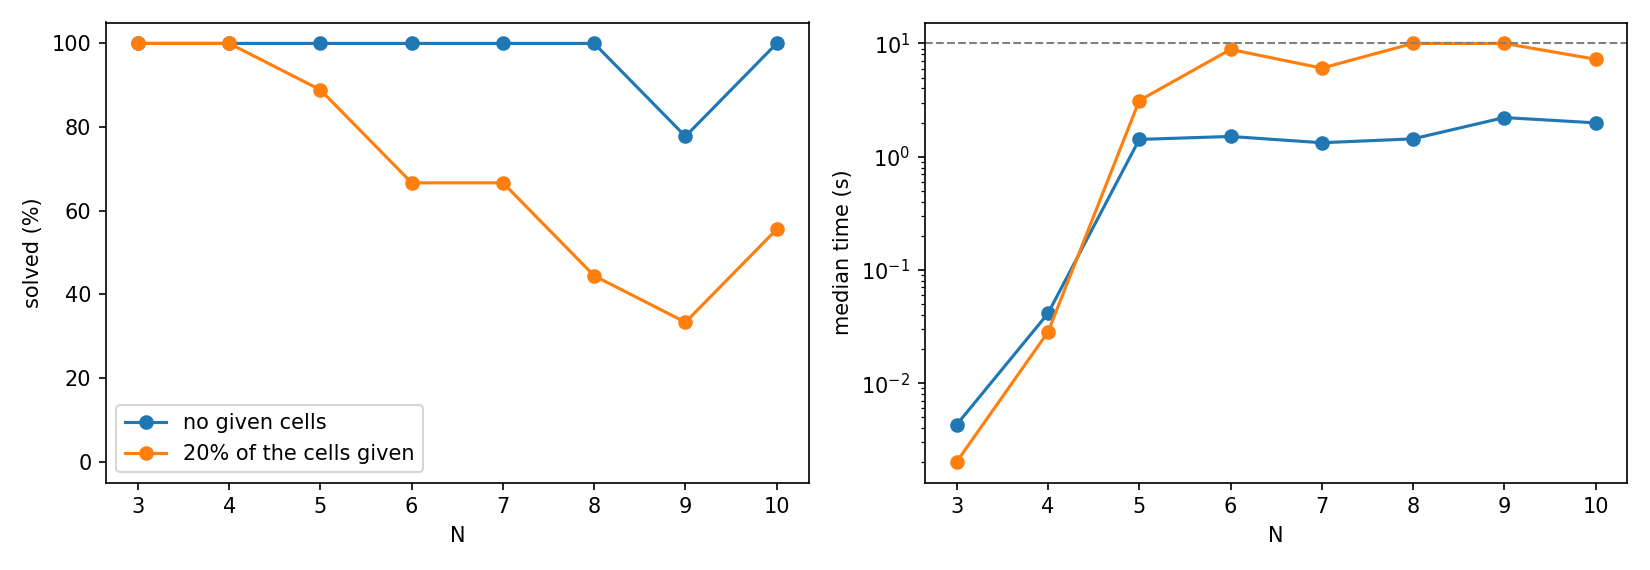
\includegraphics[width=\textwidth]{sa_time.png}
\caption{Experiment 2b: solved instances and median time (log scale);
dashed line: 10\,s limit.}
\label{fig:satime}
\end{figure}

\textbf{Analysis.}
\begin{itemize}[nosep]
  \item Without givens, SA solves every run up to $N=8$ and at $N=10$,
        and 7 of 9 at $N=9$, with a median time of at most 2.2\,s.
  \item Given cells make SA much weaker: from $N=5$ some runs fail, and at
        $N=8$--$10$ only 33--56\% are solved.
  \item From $N=5$ most runs need several restarts (median 2--7 without
        givens, 9--33 with givens): a single annealing run often ends in a
        local minimum.
  \item With only 9 runs per point, one run more or less changes the
        rate by 11\%, so the differences between $N=8$, $9$ and $10$
        are not reliable.
\end{itemize}

\section{Method 3: Genetic Algorithms}
\label{sec:m3}

\subsection{Encoding and fitness}

A genetic algorithm \cite{slides,goldberg} keeps a population of $k$
states and builds new states by combining two parents. Each state is a string over a finite
alphabet, and a fitness function gives higher values to better states.
\begin{itemize}[nosep]
  \item \textbf{encoding:} the values written in the free cells, read row
        by row; the given cells are fixed and not part of the string;
  \item \textbf{fitness:} $\phi(s)=1/(1+f(s))$, where $f$ is the energy of
        Method 2, so $\phi(s)=1$ if and only if $s$ is a magic square.
\end{itemize}

\subsection{Genetic operators}

Each generation is produced by selection, crossover and mutation:
\begin{itemize}[nosep]
  \item \textbf{selection (roulette wheel):} individual $i$ enters the
        mating pool with probability $p_i=\phi_i/\sum_k \phi_k$;
  \item \textbf{crossover:} with probability $p_c$, two parents are cut at
        a random point and their right parts are swapped. A value may then
        appear twice, so each repeated value is replaced by a missing one;
  \item \textbf{mutation:} in each child, with probability $p_m$, two
        positions of the string are swapped, so the string stays a permutation;
  \item \textbf{restart:} if the best energy does not improve for 300
        generations, the population is replaced by a new random one.
\end{itemize}
I use $k=200$, $p_c=0.9$ and $p_m=0.3$.

\textbf{Library version.} I also tried the PyGAD library (version
3.5.0) for selection, crossover and the generation loop, and kept my
own implementation because it gave worse results. PyGAD's own handling
of repeated values was too slow, and its swap mutation always exchanges
the same pair of positions, so my repair and mutation were still needed.
With them, the library version solved the $4\times4$ instance of
Experiment~3a in 8.96\,s against 3.08\,s for my code on the same
machine, since its selection and crossover are slower Python loops.

\begin{algorithm}[H]
\small
\caption{Genetic algorithm}
\label{alg:ga}
\begin{algorithmic}[1]
\Function{GeneticAlgorithm}{$G, g$}
  \State $P\gets k$ random strings (the free values shuffled)
  \Repeat
    \If{some $s\in P$ has $f(s)=0$} \State \Return $s$ \EndIf
    \If{no improvement for 300 generations} \State $P\gets k$ new random strings \EndIf
    \State $pool\gets k$ individuals drawn from $P$ with probability $p_i$
    \For{each pair $(p_1,p_2)$ in $pool$}
      \State $c_1\gets p_1$, $c_2\gets p_2$
      \State with probability $p_c$: $(c_1,c_2)\gets$ \Call{Crossover}{$p_1,p_2$}, then repair
      \State for each child $c\in\{c_1,c_2\}$, with probability $p_m$: swap two positions in $c$
    \EndFor
    \State $P\gets$ the $k$ children
  \Until{time limit reached}
  \State \Return failure
\EndFunction
\end{algorithmic}
\end{algorithm}

\subsection{Properties}
\label{sec:gaprops}

\begin{itemize}[nosep]
  \item \textbf{Not complete:} like SA, the search is random and cannot
        prove that a set of givens has no solution.
  \item \textbf{Cost per generation:} computing the fitness needs the
        $2N+2$ line sums of each of the $k$ individuals, $O(kN^2)$ in
        principle. My implementation uses a dense matrix
        multiplication, which costs $O(kN^3)$ per generation; summing the
        rows, columns and diagonals directly would reduce it to $O(kN^2)$.
  \item \textbf{Weak selection:} with $\phi=1/(1+f)$ the selection
        probability depends little on the energy when the energies are
        close. For example, in a population with energies between 2 and 12
        the best individual gets about 2 expected copies in a mating pool
        of $k$, and an individual with energy 12 about 0.5.
  \item \textbf{No elitism:} a copy of the best individual reaches the
        next generation unchanged only if there is no crossover and no
        mutation, with probability $(1-p_c)(1-p_m)=0.1\cdot0.7=0.07$. With
        about 2 copies, the best grid survives only about 13\% of the
        time, so good states are often lost.
  \item \textbf{Crossover on permutations:} the right part of one parent
        is placed in a different context, and the repair changes further
        values, so good lines of the parents are often destroyed.
  \item \textbf{Memory:} the population, $O(kN^2)$.
\end{itemize}

\noindent From these properties I expect that:
\begin{itemize}[nosep]
  \item the best energy may stop improving for long periods, because good
        states are selected weakly and often lost, so restarts are needed;
  \item the GA solves only small squares; preliminary runs suggest it is
        weaker than SA on this problem.
\end{itemize}

\subsection{Experimental setup}

The instances are built as for Method 1.

\textbf{Experiment 3a.} The $4\times4$ instance of Experiment 1a, solved
once; I record the best energy in the population at each generation.

\textbf{Experiment 3b.} $N=3,\dots,7$, with no givens or $20\%$ of the
cells given; as for Method 2, 3 puzzles and 3 independent runs per puzzle
with separate seeds (9 runs per point, 90 in total), time limit 10\,s per
run, same machine as Method 1. I record the percentage solved, the median
time (failed runs take about 10\,s) and the median best energy reached.

\textbf{Why up to $N=7$.} In preliminary runs the GA solved almost no
instance with $N\ge5$, so larger sizes would only add failed runs. I stop
at $N=7$, the same range as Method 1.

\textbf{Code and data.} Folder \nolinkurl{genetic_algorithm/} of the
repository:
\begin{itemize}[nosep]
  \item notebook: \nolinkurl{genetic_algorithm.ipynb};
  \item raw results of Experiment 3b: \nolinkurl{results_ga.csv}.
\end{itemize}

\subsection{Results}

\textbf{Experiment 3a.} The $4\times4$ instance is solved in $1.72$\,s,
after $1425$ generations and $4$ restarts; the square is the same one
found by Method 1 with AC and LCV. On the same instance SA needs
$0.04$\,s.

\begin{figure}[H]
\centering
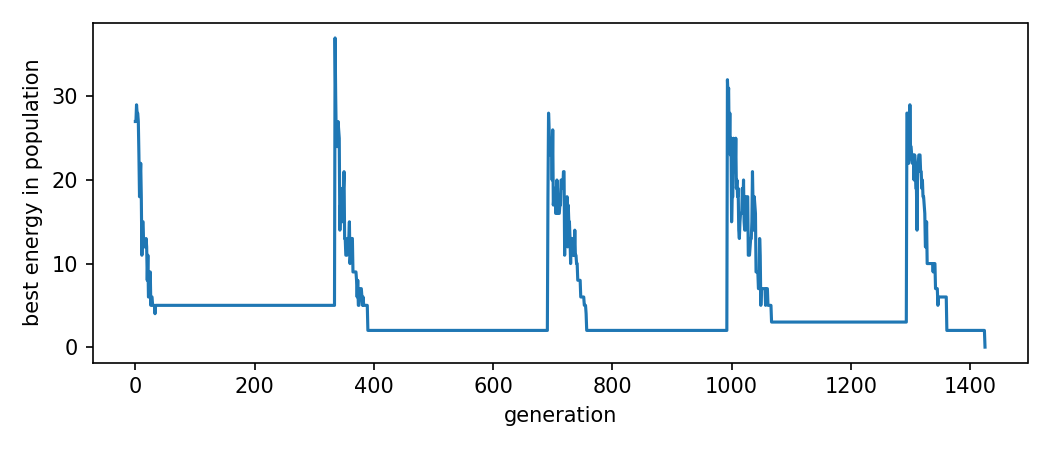
\includegraphics[width=0.75\textwidth]{ga_energy.png}
\caption{Experiment 3a: best energy in the population at each generation.
The flat parts are plateaus where the population stops improving; the
jumps are restarts.}
\label{fig:gaenergy}
\end{figure}

\textbf{Experiment 3b.}

\begin{table}[H]
\centering
\small
\begin{tabular}{@{}l rrrrr@{}}
\toprule
$N$ & 3 & 4 & 5 & 6 & 7 \\
\midrule
solved (\%), no givens   & 100 & 100 & 22 & 0 & 0 \\
solved (\%), 20\% given  & 100 & 100 & 0  & 0 & 0 \\
\midrule
median time (s), no givens  & 0.03  & 0.90 & $\geq$10 & $\geq$10 & $\geq$10 \\
median time (s), 20\% given & 0.008 & 0.55 & $\geq$10 & $\geq$10 & $\geq$10 \\
\midrule
median best energy, no givens  & 0 & 0 & 2 & 3 & 6 \\
median best energy, 20\% given & 0 & 0 & 3 & 4 & 7 \\
\midrule
median restarts, no givens  & 0 & 2 & 20 & 16 & 12 \\
median restarts, 20\% given & 0 & 1 & 22 & 18 & 14 \\
\bottomrule
\end{tabular}
\caption{Experiment 3b (9 runs per point; $\geq$10: the median run reached
the 10\,s limit; failed runs take about 10\,s). Raw
data: \nolinkurl{results_ga.csv}.}
\label{tab:ga}
\end{table}

\begin{figure}[H]
\centering
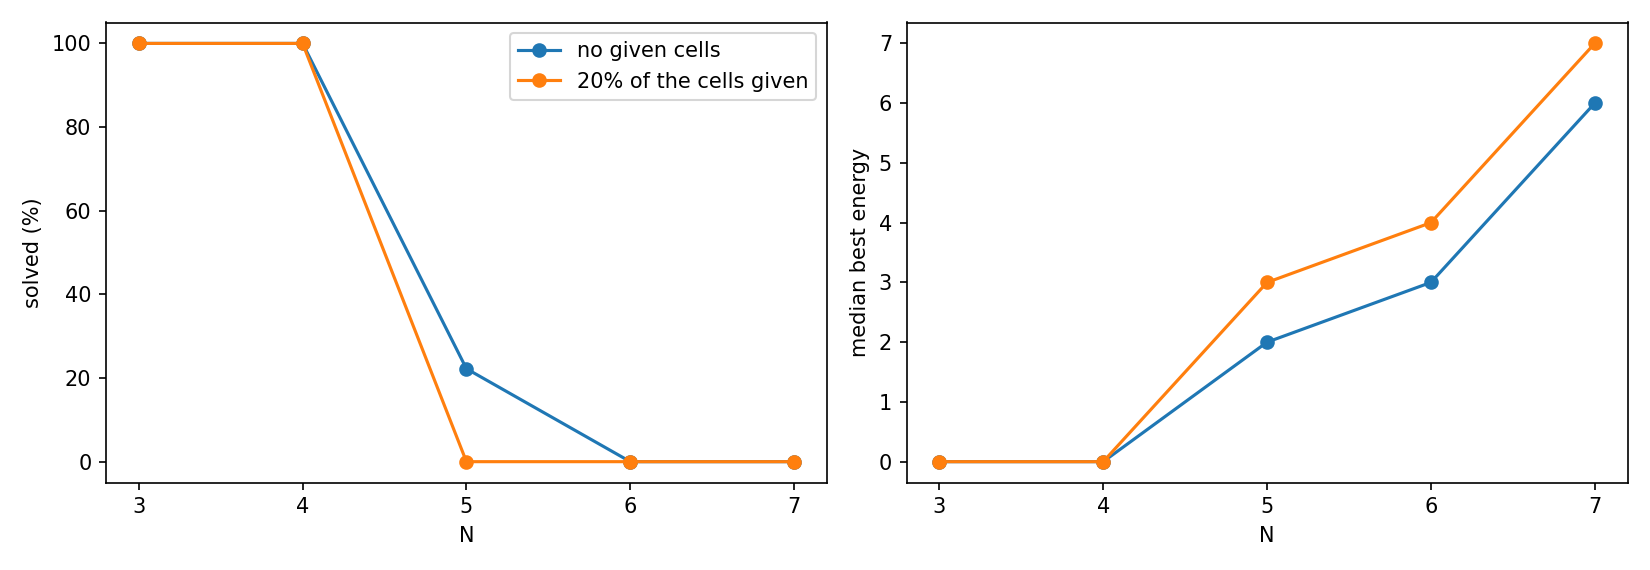
\includegraphics[width=\textwidth]{ga_results.png}
\caption{Experiment 3b: solved runs and median best energy reached.}
\label{fig:garesults}
\end{figure}

\textbf{Analysis.}
\begin{itemize}[nosep]
  \item The GA solves every run only for $N\le4$. At $N=5$ it solves 2 of
        9 runs without givens and none with givens; from $N=6$ it solves
        nothing.
  \item When it fails it still gets close: the median best energy is
        between 2 and 7.
  \item Restarts are frequent (median 12--22 for $N\ge5$), and the energy
        plot shows long plateaus where the best energy does not change.
        Loss of diversity in the population is a possible explanation, but
        I did not measure it.
  \item Even when it succeeds it is slow: on the $4\times4$ instance it
        takes about 50 times longer than SA.
\end{itemize}
On these instances the GA is the weakest of the three methods. The
properties of Section~\ref{sec:gaprops} explain it: selection barely favours the best
individuals, the best grid survives a generation only about 13\% of the
time, and crossover with repair breaks lines that the parents had right.
The search is therefore close to a random search near the current
population, which matches the long plateaus of Figure~\ref{fig:gaenergy}.

\section{Comparison of the three methods}
\label{sec:compare}

\subsection{Experimental setup}

No new runs are needed: I compare the results of Experiments 1b, 2b and
3b on the instances that all three share.
\begin{itemize}[nosep]
  \item sizes $N=3,\dots,7$, with no givens or $20\%$ of the cells given;
  \item the same puzzles (seeds $0,1,2$), the same 10\,s limit and the
        same machine;
  \item Method 1 with AC and LCV, its best setting; it is deterministic,
        so it has one run per puzzle, while SA and GA have three;
  \item failed runs take about 10\,s, as in the previous sections.
\end{itemize}
I report solved runs out of the total and the median time. The tables
are computed by the notebook \nolinkurl{comparison/comparison.ipynb}.
These are 3 of the 5 puzzles of Experiment 1b. For example, at $N=7$
with givens backtracking solves all 3 shared puzzles (100\%), while
Table~\ref{tab:alg1n} reports 60\% on all 5: the two numbers refer to
different puzzle sets.

\subsection{Results}

\begin{table}[H]
\centering
\small
\begin{tabular}{@{}cc ccc@{}}
\toprule
$N$ & givens & Backtracking (AC + LCV) & Simulated annealing & Genetic algorithm \\
\midrule
3 & no  & 3/3 & 9/9 & 9/9 \\
4 & no  & 3/3 & 9/9 & 9/9 \\
5 & no  & 3/3 & 9/9 & 2/9 \\
6 & no  & 3/3 & 9/9 & 0/9 \\
7 & no  & 0/3 & 9/9 & 0/9 \\
\midrule
3 & 20\% & 3/3 & 9/9 & 9/9 \\
4 & 20\% & 3/3 & 9/9 & 9/9 \\
5 & 20\% & 3/3 & 8/9 & 0/9 \\
6 & 20\% & 3/3 & 6/9 & 0/9 \\
7 & 20\% & 3/3 & 6/9 & 0/9 \\
\bottomrule
\end{tabular}
\caption{Solved runs on the shared instances (3 puzzles per point;
backtracking 1 run per puzzle, SA and GA 3 runs per puzzle).}
\label{tab:compare}
\end{table}

\begin{table}[H]
\centering
\small
\begin{tabular}{@{}cc ccc@{}}
\toprule
$N$ & givens & Backtracking (AC + LCV) & Simulated annealing & Genetic algorithm \\
\midrule
3 & no  & 0.007 & 0.004 & 0.03 \\
4 & no  & 0.062 & 0.04  & 0.90 \\
5 & no  & 0.22  & 1.42  & $\geq$10 \\
6 & no  & 0.47  & 1.51  & $\geq$10 \\
7 & no  & $\geq$10 & 1.33  & $\geq$10 \\
\midrule
3 & 20\% & 0.001 & 0.002 & 0.008 \\
4 & 20\% & 0.006 & 0.03  & 0.55 \\
5 & 20\% & 1.23  & 3.13  & $\geq$10 \\
6 & 20\% & 2.67  & 8.85  & $\geq$10 \\
7 & 20\% & 1.61  & 6.05  & $\geq$10 \\
\bottomrule
\end{tabular}
\caption{Median time in seconds on the shared instances ($\geq$10: the
median run reached the limit; failed runs take about 10\,s).}
\label{tab:comparetime}
\end{table}

\textbf{Analysis.}
\begin{itemize}[nosep]
  \item \textbf{Small squares ($N\le4$):} all three methods solve every
        instance; backtracking and SA in milliseconds, the GA in up to
        about 1\,s.
  \item \textbf{No givens:} backtracking solves up to $N=6$, SA solves
        most runs at every size tested (up to $N=10$ in Experiment 2b),
        the GA solves every run only up to $N=4$ (and 2 of 9 at $N=5$).
  \item \textbf{With givens:} backtracking solves all shared puzzles up to
        $N=7$, while SA fails some runs from $N=5$ and the GA solves
        nothing from $N=5$. SA and GA keep the givens fixed, and the
        givens count in the line sums, but unlike backtracking they cannot
        use them to prune the values of the other cells.
  \item \textbf{Few runs:} with only 3 puzzles per point, small
        differences are not reliable; only large ones are clear, such as
        SA (9/9) against the GA (0/9) at $N=6$ and $7$.
  \item \textbf{Time:} without givens, backtracking is faster than SA at
        $N=5,6$ (0.22\,s against 1.42\,s, 0.47\,s against 1.51\,s), but it
        stops at $N=7$, while SA keeps a median below 2\,s.
\end{itemize}

\textbf{Theory against evidence.} Table~\ref{tab:theory} puts the
properties from the theory next to what the experiments showed.

\begin{table}[H]
\centering
\small
\begin{tabular}{@{}>{\raggedright\arraybackslash}p{3.1cm} >{\raggedright\arraybackslash}p{3.9cm} >{\raggedright\arraybackslash}p{3.6cm} >{\raggedright\arraybackslash}p{3.6cm}@{}}
\toprule
Property & Backtracking (AC\,+\,LCV) & Simulated annealing & Genetic algorithm \\
\midrule
\addlinespace[2pt]
Complete & yes; solves every shared puzzle it finishes & no; needs restarts & no; needs restarts \\[3pt]
Proves ``no solution'' & yes; 0.00\,s on the impossible $3\times3$ & no; stops at the time limit & no; stops at the time limit \\[3pt]
Uses givens to prune & yes; with givens it solves $N=7$ (60\% against 0\%) & no; weaker with givens (44\% against 100\% at $N=8$) & no; 0/9 from $N=5$ with givens \\[3pt]
Memory & $O(N^6)$ worst case & $O(N^2)$ & $O(kN^2)$ \\[3pt]
Cost per step & one propagation per node, one per value with LCV & constant per swap & $O(kN^3)$ per generation \\[3pt]
Largest $N$ with every run solved, no givens & 6 & 8 (and 10) & 4 \\
\bottomrule
\end{tabular}
\caption{Properties from the theory and the evidence from the experiments
(Tables~\ref{tab:alg1n}, \ref{tab:sa}, \ref{tab:ga}, \ref{tab:checks}).}
\label{tab:theory}
\end{table}

\subsection{Correctness checks}
\label{sec:checks}

The last cells of each notebook test special cases with a 2\,s limit.
Before the search, every method checks the givens and rejects a
repeated value or a value outside $1,\dots,N^2$. Every returned square
is then checked by a separate function, written without the solver's
code: all of $1,\dots,N^2$ used once, every line summing to $M$, and the
givens kept.

\begin{table}[H]
\centering
\small
\begin{tabular}{@{}l ccc@{}}
\toprule
Case & Backtracking & Simulated annealing & Genetic algorithm \\
\midrule
repeated given ($3\times3$)          & invalid input & invalid input & invalid input \\
given out of range ($3\times3$)      & invalid input & invalid input & invalid input \\
centre $=1$ ($3\times3$, no solution) & no solution, 0.00\,s & time limit & time limit \\
complete $4\times4$ square           & solved & solved & solved \\
1 or 2 empty cells ($4\times4$)      & solved & solved & solved \\
random puzzles, $N=3,4$              & 20/20 & 20/20 & 19/20 \\
\bottomrule
\end{tabular}
\caption{Correctness checks (2\,s limit). Every square returned passed the
separate check; the random puzzles are seeds $0,\dots,4$ with no givens or
$20\%$ given.}
\label{tab:checks}
\end{table}

\noindent The impossible case shows the difference stated by the theory:
backtracking proves at once that there is no solution, while SA and the
GA cannot tell an impossible puzzle from a hard one and stop only at the
time limit.

\section{Conclusions}
\label{sec:conclusions}

\begin{itemize}[nosep]
  \item \textbf{Backtracking} is exact and complete, as the theory says.
        AC with LCV reduced the search a lot compared with FC with ascending
        order (394 nodes at $N=5$, while FC with ascending order explores about
        1.2 million nodes in 10\,s without a solution), but the time still grows exponentially:
        without givens it stops at $N=6$.
  \item \textbf{Simulated annealing} is not complete, but it scaled
        furthest in these experiments: up to $N=10$ without givens, with a
        median time of at most 2.2\,s. The cheap evaluation of each swap (stored
        line sums, updated only on the changed lines) and its ability to leave local minima,
        by accepting worse moves and restarting, are plausible reasons. Given cells made
        it weaker: it keeps them fixed but, unlike backtracking, cannot use
        them to prune the other values.
  \item \textbf{The genetic algorithm} was the weakest: it solved every
        run only up to $N=4$, and 2 of 9 runs at $N=5$. With roulette
        selection on $\phi=1/(1+f)$ and no elitism, good grids are selected
        weakly and usually lost (the best survives a generation about 13\%
        of the time), and crossover on permutations breaks lines that were
        already correct.
\end{itemize}

In short, on the tested cases backtracking is the better choice for
small squares, when 20\% of the cells are given, or to prove that there
is no solution; simulated annealing is the better choice for larger
squares without givens. These results come
from few runs per point and a 10\,s limit, so they show trends rather than
exact values.

\begin{thebibliography}{9}
\bibitem{slides} A.~Torsello, \emph{Foundations of Artificial
  Intelligence}, lecture slides: Blind Search, Constraint Satisfaction,
  Local Search. Università Ca' Foscari Venezia.
\bibitem{aima} S.~Russell, P.~Norvig, \emph{Artificial Intelligence: A
  Modern Approach}, 4th ed., Pearson, 2020.
\bibitem{kirkpatrick} S.~Kirkpatrick, C.~D.~Gelatt, M.~P.~Vecchi,
  Optimization by simulated annealing, \emph{Science} 220(4598),
  671--680, 1983.
\bibitem{goldberg} D.~E.~Goldberg, \emph{Genetic Algorithms in Search,
  Optimization and Machine Learning}, Addison-Wesley, 1989.
\end{thebibliography}

\end{document}